\section{Анализ полученных результатов теплового режима РЭС}
\subsection{Обработка и анализ данных проведенного результата}

Гораздо легче принимать конструкторские решения обладая визуальным
представлением данных. По это причине данный раздел в основном состоит
из гистогорамм отображающих в результаты расчетов температур.




\subsubsection{Анализ тепловых режимов для корпуса блока}
\begin{figure}[h] %% h means here
\begin{center}
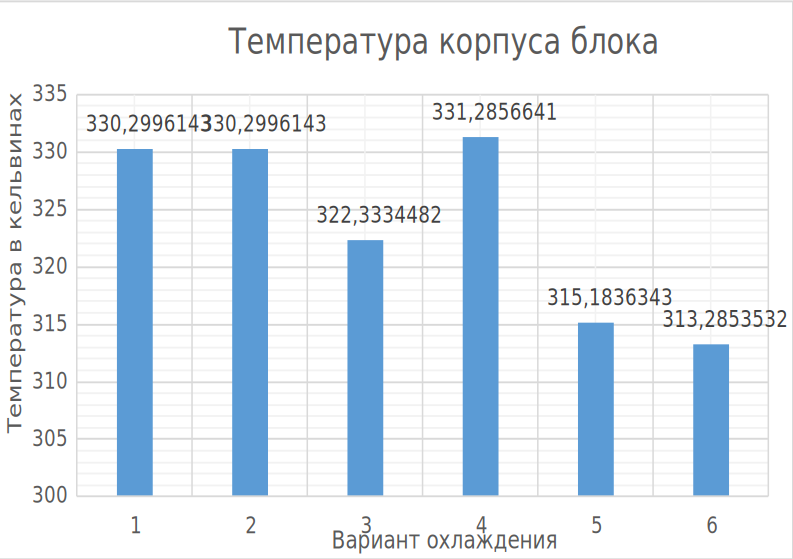
\includegraphics[scale = 0.4]{images2/t_corp.png}
\caption{Температура корпуса блока:\\
  1 - тепловой режим герметичного корпуса\\
  2 – тепловой режим блока в герметичном корпусе с внутренним перемешиванием\\
  3 – тепловой режим блока в герметичном корпусе с наружным обдувом\\
  4 - телповой режим блока в  герметичном оребренном корпусе \\
  5 – тепловой режим блока в перфорированном корпусе \\
  6 - тепловой режим блока при принудительном охлаждении}
\end{center}

\end{figure}

На гистогорамме ожидаемо оказались примерно равными значения
температур для герметичного корпуса и для корпуса с внутренним
перемешиванием. Это обусловлено тем, что скорость перемешивания при
расчете была равна нулю и закономерно.


Неожиданно то, что значения температур при использовании
оребренного корпуса оказались самыми большими.
Это может свидетельствовать об ошибках в расчетах.

Так же неожиданно столь низкая температура,
при использовании принудительного охлаждения.
Однако, вполне ожидаемо, что при принудительном
температура корпуса будет самой низкой.

Самым эффективным длия отвода тепла, после использования
принудительного охлаждения, оказалось использование перфорированного
корпуса.

\subsubsection{Анализ тепловых режимов нагретой зоны}
\begin{figure}[h]
  \begin{center}
    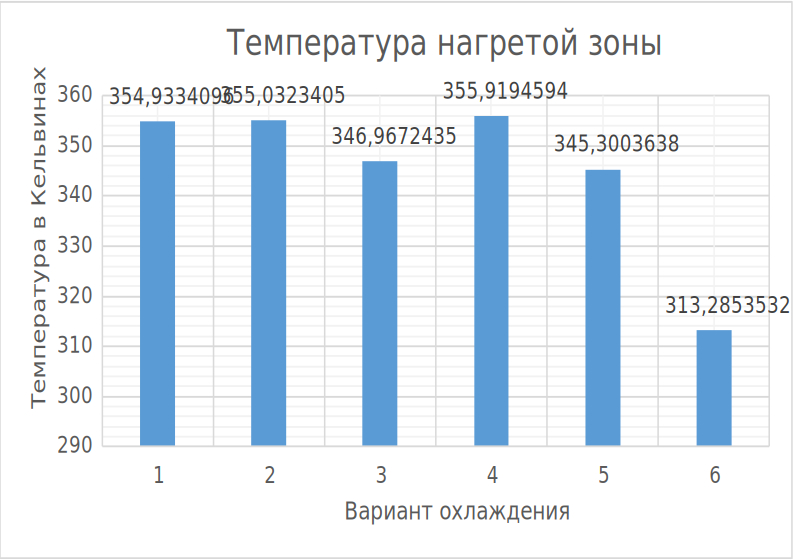
\includegraphics[scale=0.4]{images2/t_surface.png}
\caption{Температура поверхности элемента:\\
  1 - тепловой режим герметичного корпуса\\
  2 – тепловой режим блока в герметичном корпусе с внутренним перемешиванием\\
  3 – тепловой режим блока в герметичном корпусе с наружным обдувом\\
  4 - телповой режим блока в  герметичном оребренном корпусе \\
  5 – тепловой режим блока в перфорированном корпусе \\
  6 - тепловой режим блока при принудительном охлаждении}
    
   \end{center}
 \end{figure}

 Температуры нагретой зоны, при использовании
 герметичного корпуса, корпуса с внутренним перемешиваением и
 оребрённого корпуса оказываются примерно одинаковыми.

 Cамыми низкими окызываются температуры при
 использовании принудительного воздушного охлаждения,
 при использовании перфорированного корпуса и
 при обдуве корпуса.
 
\subsubsection{Анализ тепловых режимов для поверхности элемента}
\begin{figure}[h] %% h means here
\begin{center}
  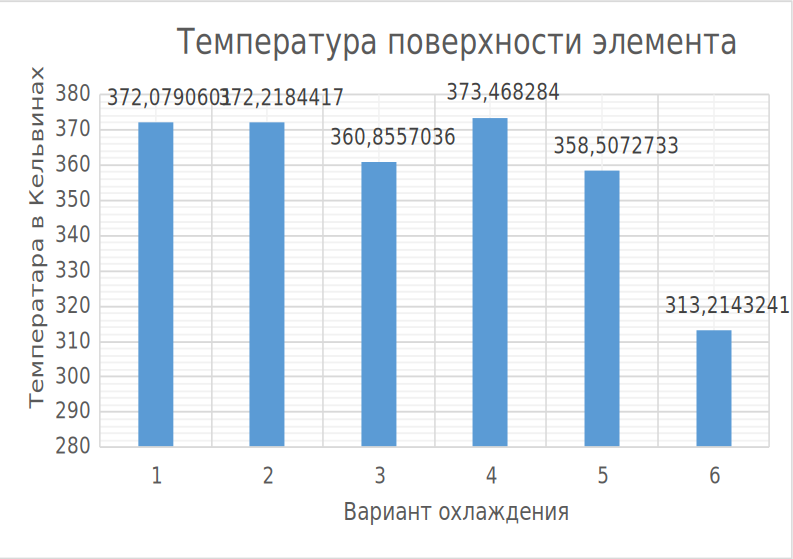
\includegraphics[scale = 0.4]{images2/t_el.png}
  \end{center}
\caption{Температура поверхности элемента:\\
  1 - тепловой режим герметичного корпуса\\
  2 – тепловой режим блока в герметичном корпусе с внутренним перемешиванием\\
  3 – тепловой режим блока в герметичном корпусе с наружным обдувом\\
  4 - телповой режим блока в  герметичном оребренном корпусе \\
  5 – тепловой режим блока в перфорированном корпусе \\
  6 - тепловой режим блока при принудительном охлаждении}

\end{figure}

Ожидаемое самым низким оказалась температура в телповом режиме с
принудительным охлажденим. Возможно, даже слишком низкой и в расчетах
присуствует ошибка.\\

Вновь самой большой оказалась температура при использовании оребренного коруса.\\

Самыми низкой температурой поверхность обладала при использовании
перфорации.\\

При использовании обдува температура оказалось чуть выше.\\

Снова можно говорить о том, что,
после использовани принудительного
охлаждения,
самым эффективным является использование перфорации,
а за ним идёт использовании корпуса с наружным обдувом.

\subsubsection{Анализ тепловых режимов для воздуха в блоке.}
\begin{figure}[h] %% h means here
\begin{center}
  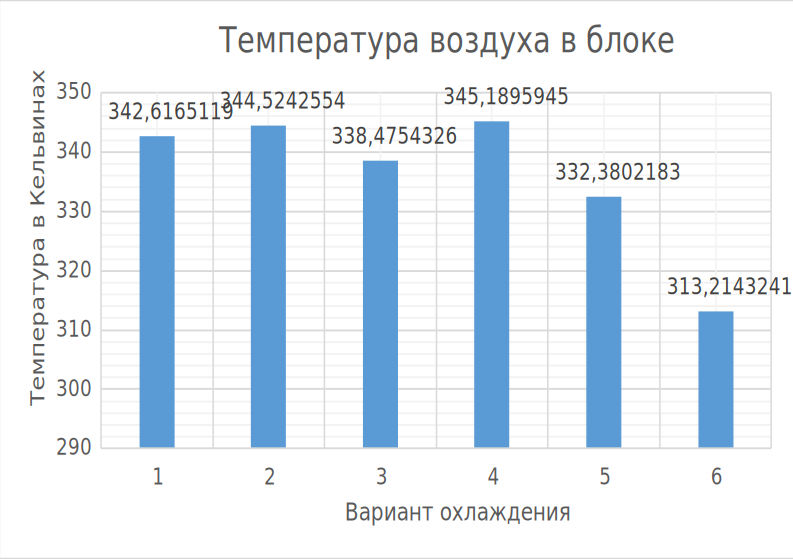
\includegraphics[scale = 0.4]{images2/t_air.png}
  \end{center}
\caption{Температура воздуха блоке:\\
  1 - тепловой режим герметичного корпуса\\
  2 – тепловой режим блока в герметичном корпусе с внутренним перемешиванием\\
  3 – тепловой режим блока в герметичном корпусе с наружным обдувом\\
  4 - телповой режим блока в  герметичном оребренном корпусе \\
  5 – тепловой режим блока в перфорированном корпусе \\
  6 - тепловой режим блока при принудительном охлаждении}

\end{figure}

На данной графике самым эффективным оказывается режим с принудительным
воздушным охлажденим, что закономерно.

Однако, на графике видно, что при перемешивании температура воздуха
выше, чем при его отсуствии на два градуса, что может
свидетельствовать об ошибке в вычислениях.

В прочем, сложно сказать достоверно ли это, так как при расчете
скорость перемешивания взята равной нулю, что обусловлено тем, что
охлаждение естественное.


На этом этапе становится анализа становятся очевидн
\begin{enumerate}[label={\arabic*.}]

\item Самое эффективный способ охлаждения из рассмотренных
  — принудительное воздушное охлаждение.
\item Значения первых двух тепловых режимов, то есть теплового режима
  герметичного корпуса и герметичного корпуса с перемешиванием в
  большинстве случаев будут выше чем значения в остальных температурных режимах.

\item Самым эффективным после принудительного воздушного охлаждения,
  является метод использования перфорированного корпуса или внешнего
  обдува.
\end{enumerate}

Это означает, что, если исключить вариант принудительного воздушного
охлаждения, то по сути решение инженерной задачи это выбор между
использованием корпуса с перфорацией и внешним обдувом корпуса.


\subsubsection{ Анализ тепловых режимов окружающей элемент среды.}
\begin{figure}[h] %% h means here
\begin{center}
  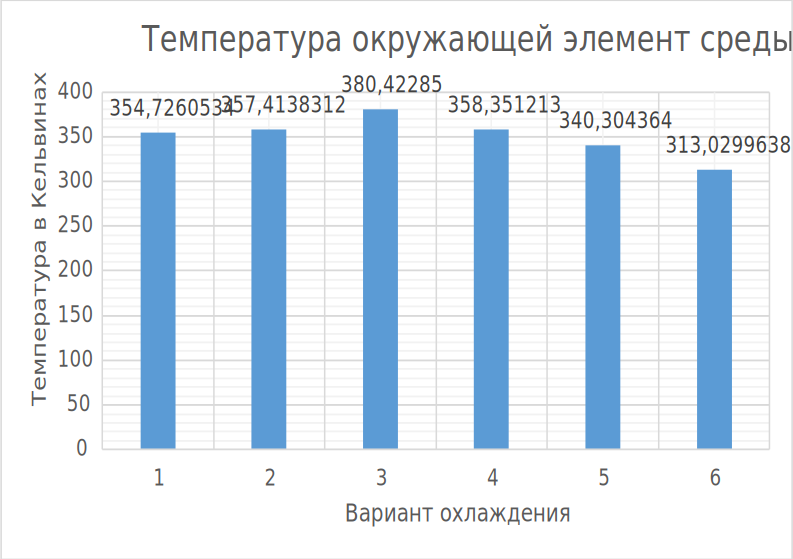
\includegraphics[scale = 0.4]{images2/t_env.png}
  \end{center}
\caption{Температура окружающей элемент среды:\\
  1 - тепловой режим герметичного корпуса\\
  2 – тепловой режим блока в герметичном корпусе с внутренним перемешиванием\\
  3 – тепловой режим блока в герметичном корпусе с наружным обдувом\\
  4 - телповой режим блока в  герметичном оребренном корпусе \\
  5 – тепловой режим блока в перфорированном корпусе \\
  6 - тепловой режим блока при принудительном охлаждении}

\end{figure}

Данная гистограмма выглядит, как наиболее близкая к действительным
значениям, если не считать, что на ней самой большой температурой
окружающая среда элемента обладает в случае использования наружного
обдува.

Закономерно, вновь самыми низкими являются температуры при принудительном охлаждении
и при использовании перфорированного корпуса.


\subsubsection{Моделирование теплового режима в elcut}

На основании полученных данных была создана модель печатной платы в
elcut.

Точнее будет сказать, что была создана стационарная задача
теплопроводности, в которой была создана геометрия печатной платы и
расчитываемого элемента.

\begin{figure}[h]
  \centering
  \includegraphics[scale = 0.40]{images2/elcut_model.png}
  \caption{ Созданная в elcut геометрия печатной платы и процессора. }
\end{figure}

На приложенно иллюстрации видно, что созданы метки блоков
для процессора и печатной платы.

Однако в метках блока возможно указать только теплопроводность, а не
температуру или рассеиваемую мощность. Это обусловлено спецификой
программы и использования метода конечных элементов.

\begin{figure}[h]
  \centering
  \includegraphics[scale = 0.40]{images2/Elcut_cpu_lambda.png}
  \caption{ Установка значений теплопроводности для метки блока CPU }
\end{figure}

Для метки блока процессора было установлено значение теплопроводности
соответсвующие таковому у аллюминия.

\begin{figure}[h]
  \centering
  \includegraphics[scale = 0.40]{images2/Elcut_pcb_lambda.png}
  \caption{ Установка значений теплопроводности для метки блока PCB }
\end{figure}

Для метки блока процессора было установлено значение теплопроводности
соответствующие стеклотекстолиту~\cite{teplotim}.

Далее, чтобы решить задачу стационарной теплопроводности в elcut на
вершины фигуры процессора были установлены метки с температурой
соответсвующей полученной в расчетах температуре поверхности элемента,
а на вершины фигуры печатной платы были установлены метки,
oсоответствующие температуре окружающей среды, используемой в рачетах.

\begin{figure}[h]
  \centering
  \includegraphics[scale = 0.3]{images2/elcut_calculate_with_temp_6.png}
  \caption{ Решение задачи теплопроводности для герметичного корпуса с перфорацией в elcut }
\end{figure}

На приведенной иллюстрации видно, что полученная в результате решения
задачи теплопроводности для перечисленных методов охлаждения
температура окружающей элемент поверхности
сошлась с температурой окружающей элемент поверхности полученной в
расчетах.

